\documentclass[11pt]{report}

\usepackage[utf8]{inputenc} % Required for inputting international characters
\usepackage[T1]{fontenc} % Output font encoding for international characters
\usepackage[a4paper, total={7in, 10in}]{geometry}
\usepackage{mathpazo} % Palatino font
\usepackage{graphicx}
\usepackage{sectsty}
\usepackage{lipsum} 
\usepackage{pgfgantt}
\usepackage{afterpage}
\usepackage{wrapfig}
% \usepackage{indentfirst}
\usepackage{float}
\usepackage{framed}
\usepackage[pagestyles]{titlesec}
\renewcommand\bibname{References}
% \titleformat{\chapter}{\bfseries\centering}{}{0pt}{\Huge}
\titleformat{\chapter}[display]
  {\normalfont\huge\bfseries}
  {}
  {0pt}
  {\filcenter\Huge\scshape}
\titlespacing*{\chapter}{0pt}{40pt}{40pt}
\titleformat*{\section}{\Large\bfseries}
\titleformat*{\subsection}{\large\bfseries}

\renewcommand*\footnoterule{}
% \newpagestyle{mystyle}
% {\sethead[\thepage][][\chaptertitle]{}{}{\thepage}}
% \pagestyle{mystyle}
\pagestyle{plain}
\setlength{\FrameSep}{10pt}
\setlength{\FrameRule}{1pt}
\newcommand{\HRule}{\rule{\linewidth}{1pt}\bigskip\par}
% \allsectionsfont{\centering}

\begin{document}
\begin{center}
\textbf{\LARGE\textsc{Department of Computer Science and Engineering}}\bigskip\\
\textbf{\Large{VIII Semester Project}}\bigskip\\
\textbf{\huge\textsc{Monthly Progress Report - I}}\bigskip\\
\end{center}
\begin{framed}
\noindent \large{Batch No. }\hspace{64pt}\textbf{\large{35}}\medskip\\
\large{Title of the project: }\hspace{17pt}\textbf{\large\textsc{Picture Regeneration using Generative Models}}\medskip\\
\noindent\begin{tabular}{@{}l@{\hspace{31pt}}l r }
\large{Team members: }  & {\large \textbf{Abhijith C.}}       & \large \textbf{1MV14CS004} \\
                        & {\large \textbf{Raghava G. Dhanya}} & \large \textbf{1MV14CS077} \\
                        & {\large \textbf{Shashank S.}}       & \large \textbf{1MV14CS131}
\end{tabular}\\[15pt]  
\noindent \large{Name of the Guide }\hspace{13pt}\textbf{\large{Sushila Shidnal}}\medskip\\
\noindent \large{Duration }\hspace{66pt}\textbf{\large{From sometime to sometime}}\medskip\\
\HRule
\noindent \textbf{\Large{Details Of Work Carried Out:}}\bigskip\\
\large{Under Basic GAN, we implemented the DCGAN architecture from Alec Radford \textit{et al}\footnotemark. We were able to reproduce the results on the MNIST dataset and on facial images with a high degree of visual accuracy. The training took around 30 hours to complete on a modest home computer.\par}
\begin{wrapfigure}{l}{0.3\textwidth}
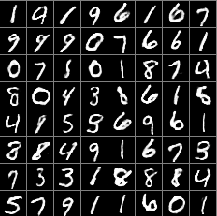
\includegraphics[width=.3\textwidth]{MNIST.png}
\caption{GAN output after 40000 epochs}
\end{wrapfigure} 
\lipsum[1-2]

\end{framed}
\footnotetext{Alec Radford, Luke Metz, and Soumith Chintala. Unsupervised representation learning with deep
convolutional generative adversarial networks. CoRR, abs/1511.06434, 2015.}
\afterpage{
\begin{framed}
\noindent \textbf{\Large{Time-line:}}\\[10pt]

\includegraphics[width=1.1\textwidth]{timeline.png}\\[10pt] 
\noindent\HRule
\vspace{50px}
\centering
\textbf{Head of the Department}
\vspace{50px}
\flushleft\textbf{Project Guide}\hfill\textbf{Project Coordinator}
\end{framed}
}
\end{document}